Nestled in the bustling heart of a glamorous city, a place where the world's most discerning travelers come to rest and recharge, stands a hotel that's both a destination and a time capsule: the Grand Hotel Infinita. It was an old, magnificent building, infinitely tall and wide, where history and luxury met. It was a place where every guest could escape the demands of the modern world and refill their energies in an environment of timeless elegance. Due to its size and age, the hotel had no passenger elevators, just an infinite number of stairs connecting all floors. To provide greater convenience, the hotel had recently installed a small, rattling freight elevator connected to every room. Guests could call the front desk to request snacks, drinks, or fresh towels, and their request would be delivered through the freight elevator.

The lobby, with its soaring ceilings, featured a sweeping marble staircase that seemed to climb forever. A massive chandelier cast a warm, golden light, creating a charming atmosphere. The front desk was a masterpiece of carved mahogany, manned by staff in impeccably tailored uniforms. At the desk sat Henrietta, a kind-hearted hippopotamus. Her assistant, Bernard, a diligent bellrat, stood by with polished luggage carts, awaiting the next guest. They were the hotel's only two staff members. With an infinite number of rooms to keep in order, they had to deal with an endless stream of guests arriving and leaving at all hours. It was a duty they fulfilled exquisitely, thanks to their superb organization and commitment to harmony.

\clearpage
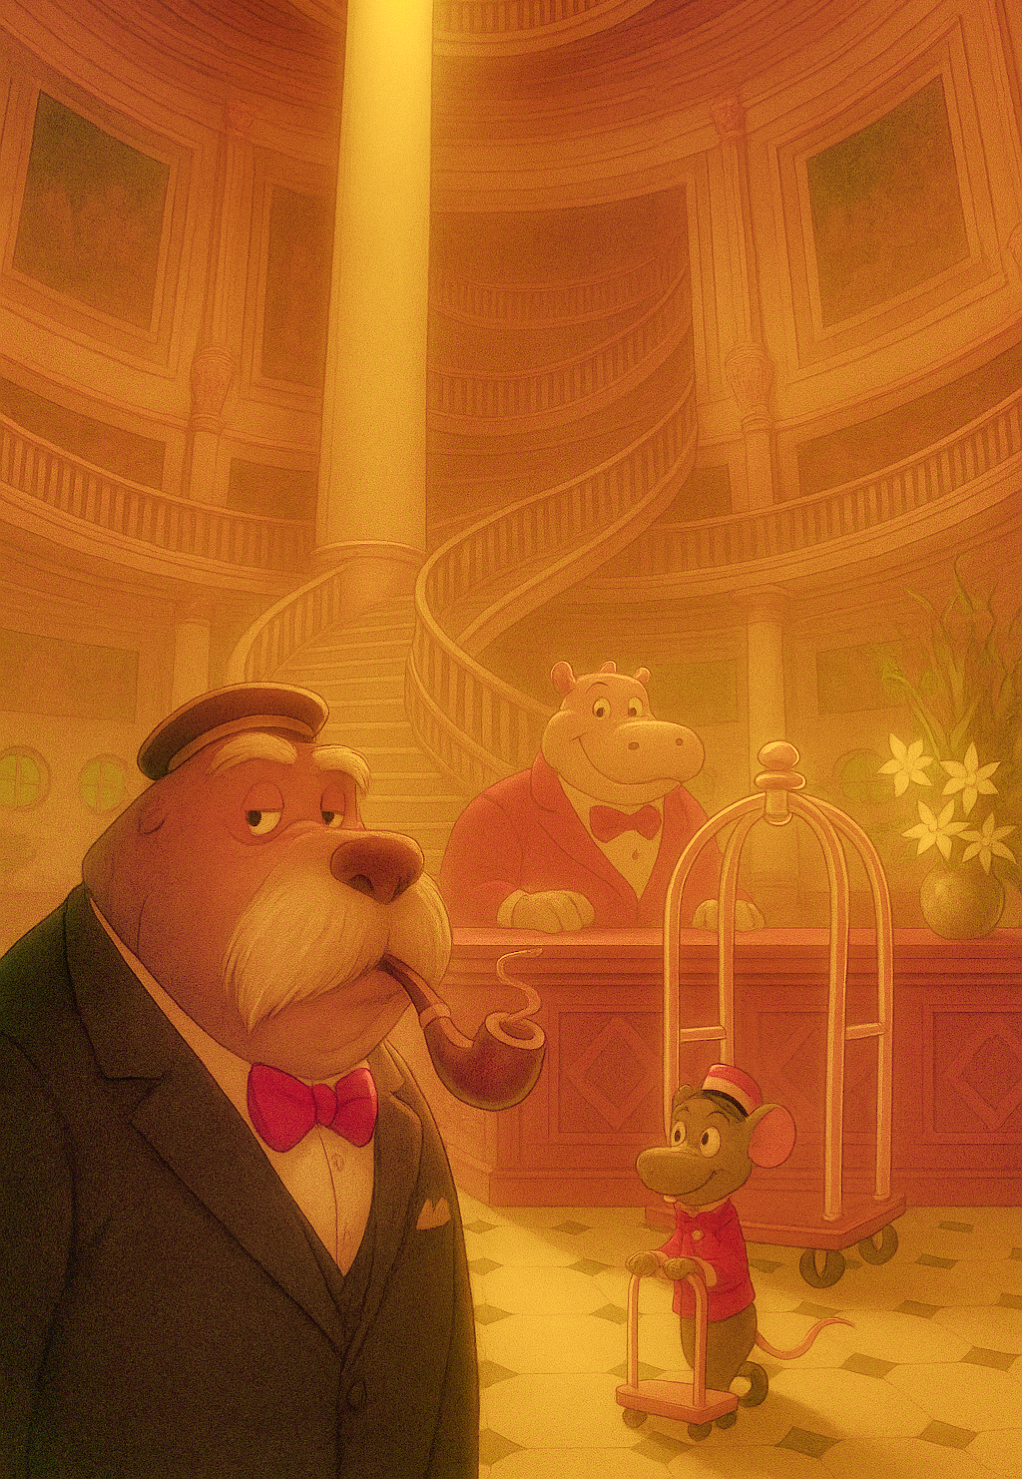
\includepdf[pages={1},
            pagecommand={\thispagestyle{fancy}}, % Apply your custom 'fancy' style
            fitpaper=true,
            noautoscale
           ]{walrus.pdf}

On the night before the holiday, a distinguished walrus smoking a pipe was the last guest to arrive. He looked terribly tired as he walked in. Henrietta, always affectionately welcoming new guests, greeted him with a wide smile.

``It's a pleasure to welcome you to the Grand Hotel Infinita,'' she said. ``A place where the longing quest is left behind, where you may rest and ease your weary mind.'' 
%``A place where the longing quest is left behind, where you may rest and leave the whirlpool of wild dreams behind.''

``Oh, that's all I need,'' the walrus replied with a sigh of relief.

``Our hotel is quite full today, but you're in luck, Mr. Walrus! The first room on the first floor just became vacant!'' Henrietta exclaimed. ``Our agile Bernard will help you to your room instantly.''

Bernard led him to his room where he enjoyed a wonderfully restful night.

\vspace{4em}
The next morning was the start of an extended national holiday, the first after a long winter. The hotel staff started the day with a special kind of excitement. They were all eager, awaiting the first wave of guests. This old, glamorous hotel was awake and ready, poised to welcome a new day and create new memories. But what should have been a time for rest and tranquility turned into a great fuss, with many guests complaining about their missing heirlooms.
